\begin{figure}[htp] \centering
    \begin{subfigure}[b]{0.96\columnwidth}
        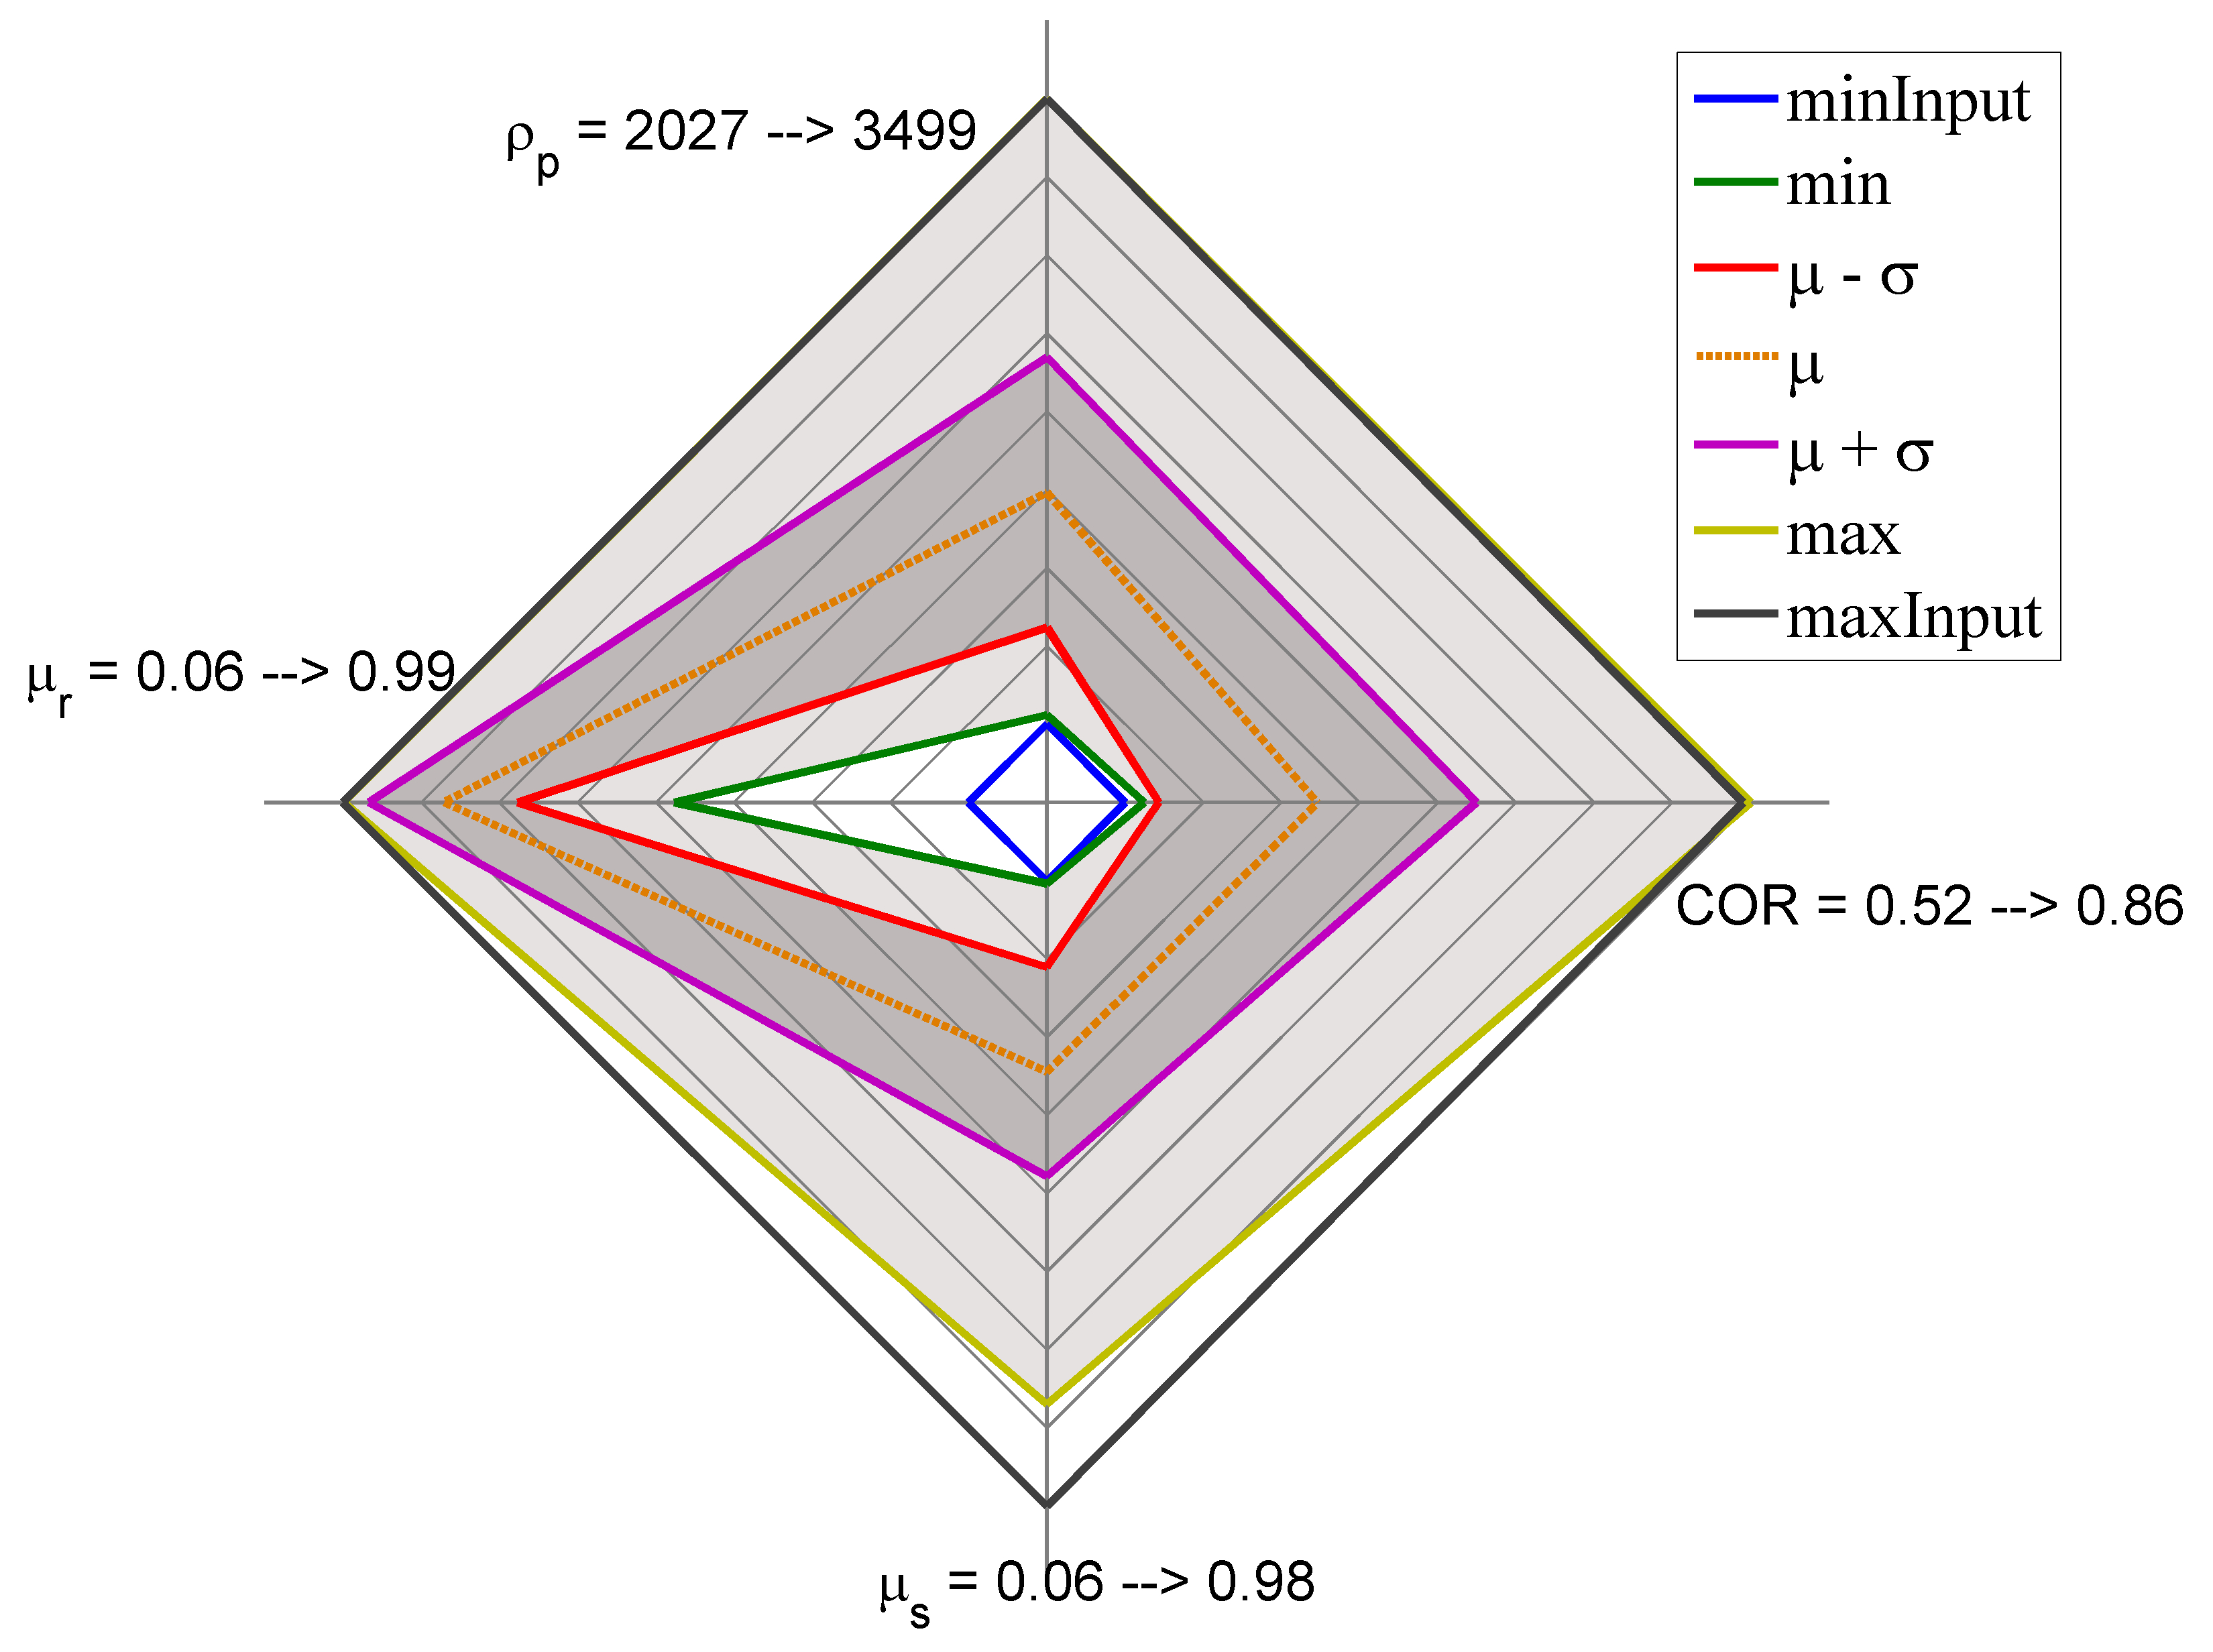
\includegraphics[width=\textwidth]{images/original/31radarpirker1aor}
        \caption{Radar plot, $AOR_{exp} = 38.85 ^\circ$}
        \label{fig:31radarpirker1aor} 
    \end{subfigure}\\
        \begin{subfigure}[b]{0.96\columnwidth}
        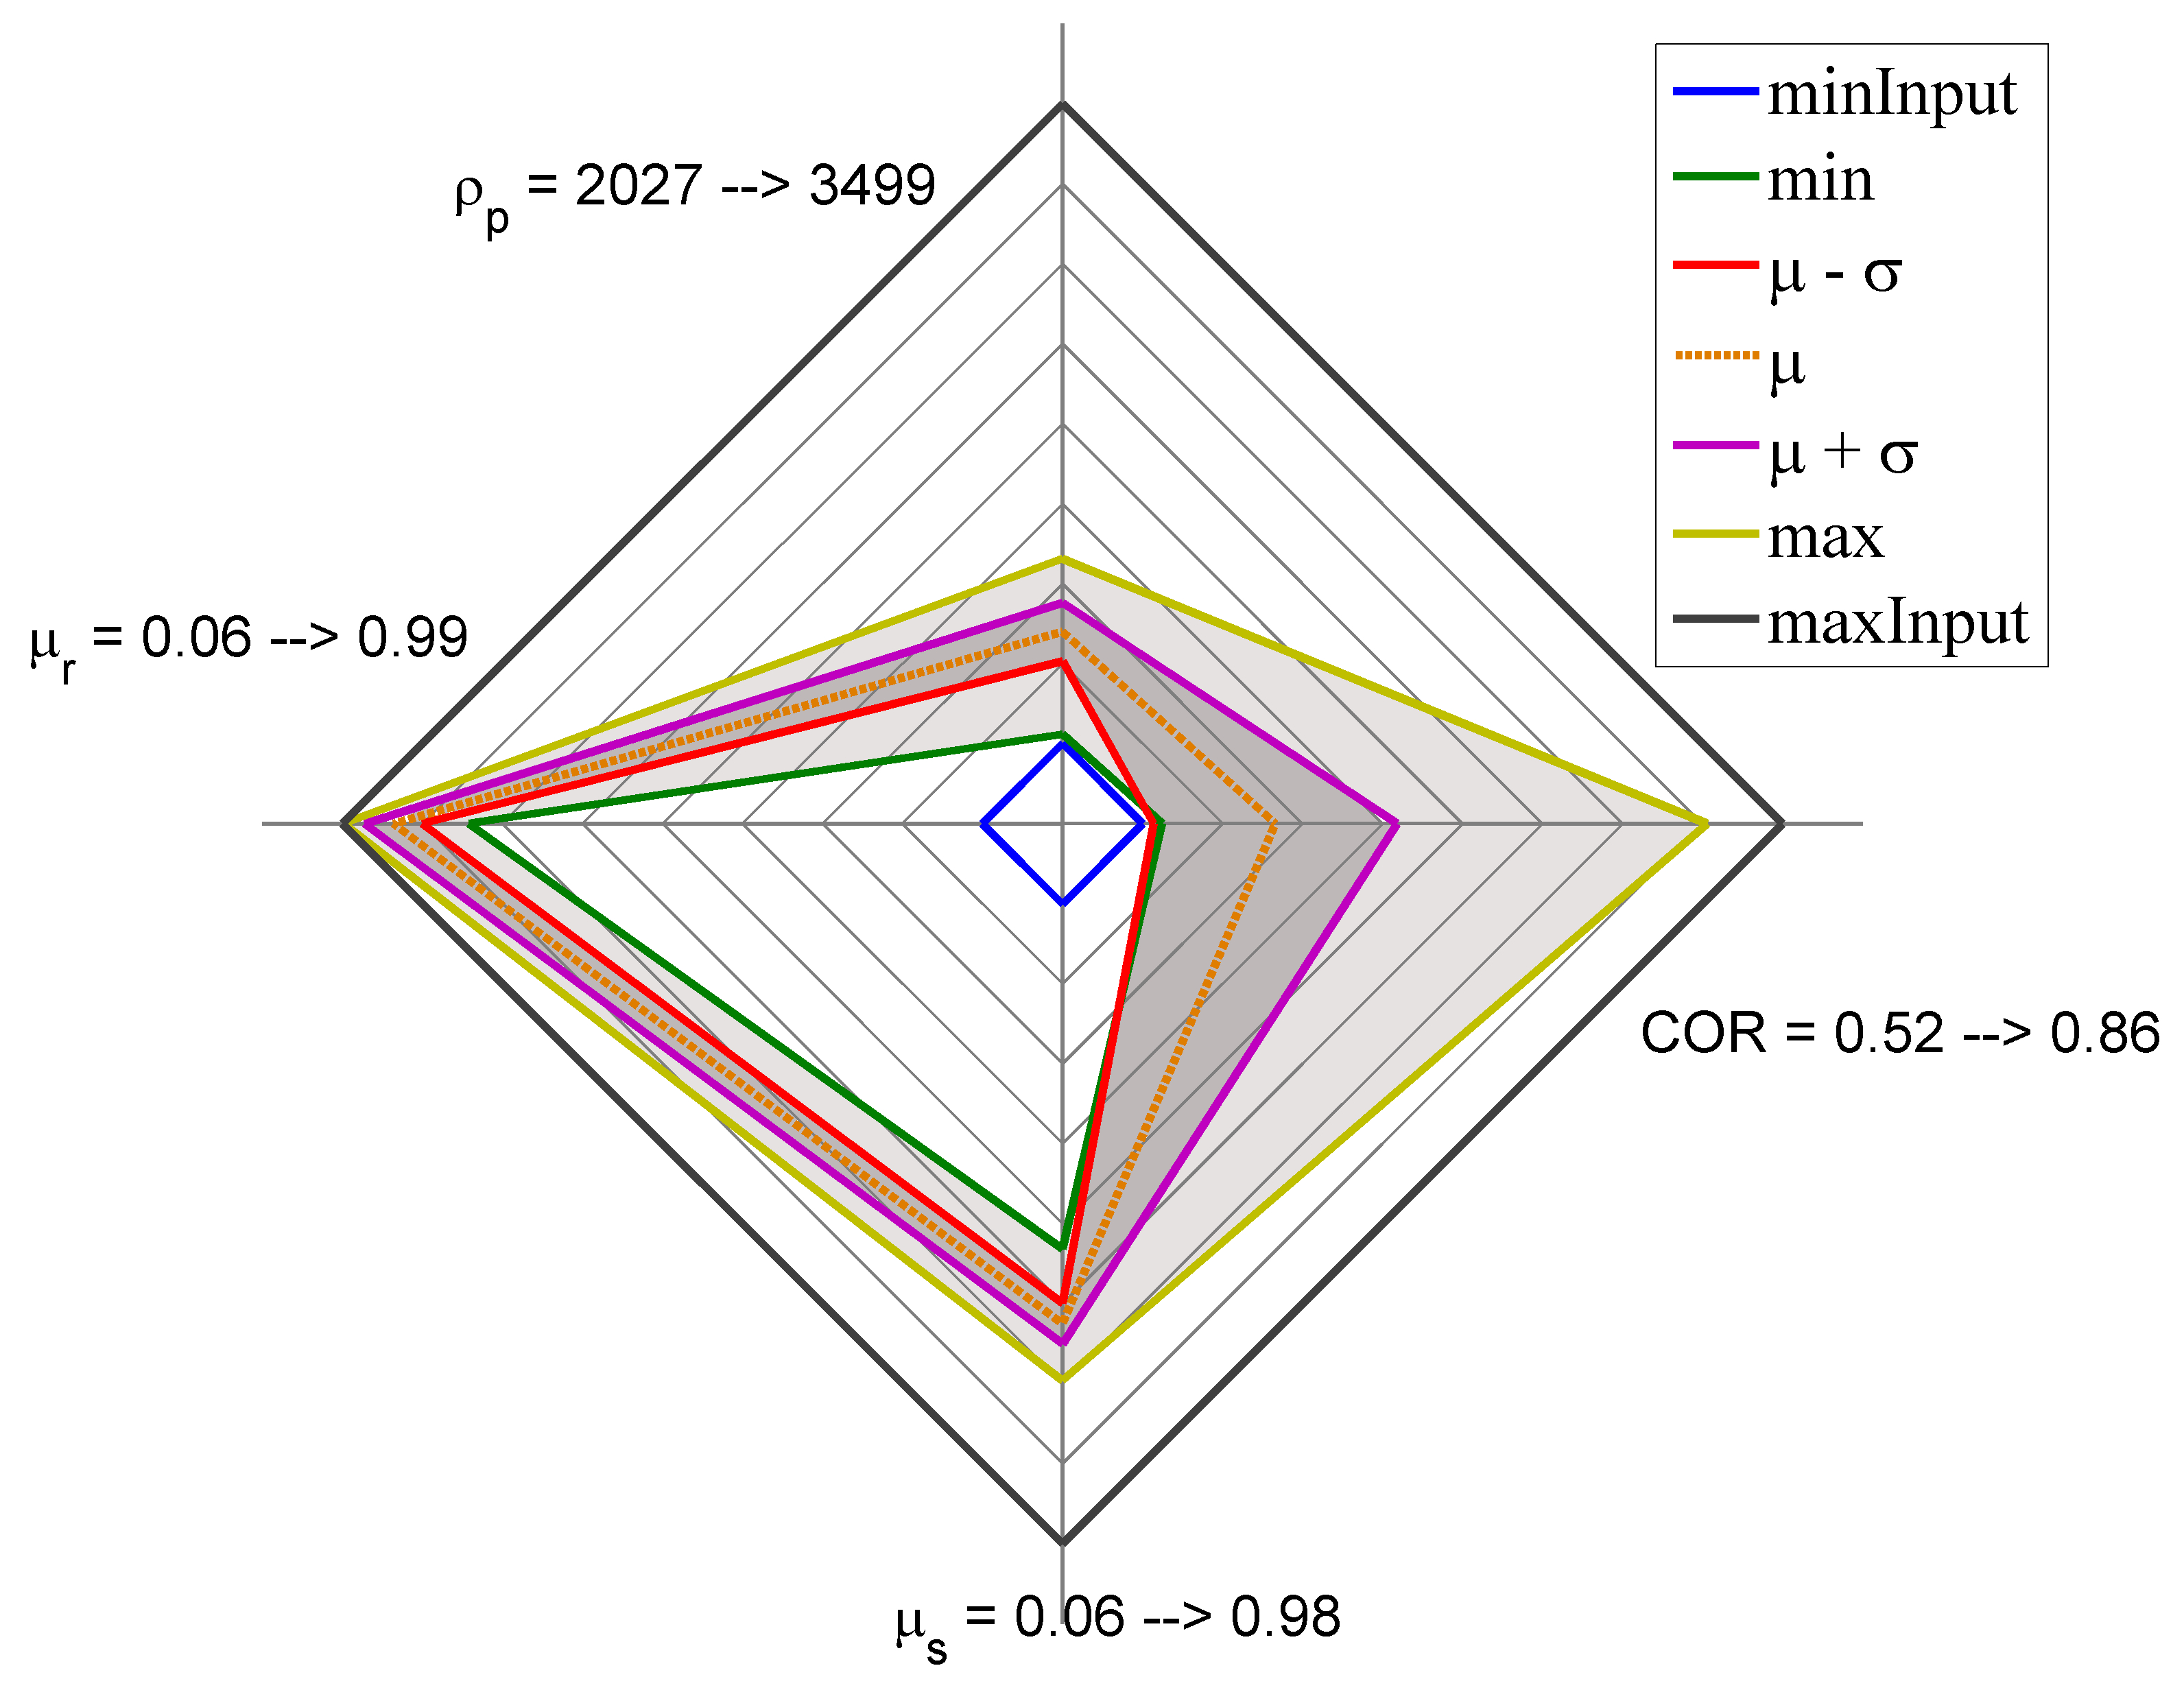
\includegraphics[width=\textwidth]{images/original/33radarpirker1schulze10070aor}
        \caption{Radar plot, $AOR_{exp} = 38.85
        ^\circ$, $SCT$, $\sigma_n=10070 ~[Pa]$}
        \label{fig:33radarpirker1schulze10070aor} 
    \end{subfigure}
    \caption[Radar plot comparison of AOR and SCT results]{Radar plot comparison
    of $AOR$ and $SCT$ results. We represent the tabbed combinations for the
    $AOR$ test.
    The minimum and maximum values, together with the mean and the confidence
	range, provided by the square deviation, are shown.
    Here, the values plotted are selected between the numerical
    values from the $NN$ with initially the original experimental results for
    the $AOR$, $P=1.0$ (Fig.
    \ref{fig:31radarpirker1aor}). 
    The confidence range is large, except for the $\mu_r$.
    The last image (Fig. \ref{fig:33radarpirker1schulze10070aor}) represents
    instead the values valid for both the $AOR$ test and the $SCT$, with a
    $\sigma_n=10070 ~[Pa]$, both for $P=1.0$.
    The range is meager, except for the $COR$.    }
    \label{fig:35schulze10070aorradarandcloud}
\end{figure}